\hsection{Problem Instance Data}%
\label{sec:problemInstance}%
%
\hsection{Definitions}%
%
We distinguish optimization \emph{problems} (see \autoref{def:optimizationProblemMathematical}) from \emph{problem instances}.
An optimization problem is the general blueprint of the tasks.
The JSSP (see \autoref{sec:jsspExample}), for instance, has the goal of scheduling production jobs to machines under a set of constraints that we will discuss later.
A problem instance of the JSSP is a concrete scenario, e.g., a concrete lists of tasks, requirements, and machines.%
%
\begin{definition}%
\label{def:instance}%
A concrete instantiation of all information that are relevant from the perspective of solving an optimization problems is called a \emph{problem instance}~\instance.%
\end{definition}%
%
The problem instance is the input of the optimization algorithms.
A problem instance is related to an optimization problem in the same way an object/instance is related to its \texttt{class} in an object-oriented programming language like Python or Java, or a \texttt{struct} in~C.
The \texttt{class} defines which member variables exists and what their valid ranges are.
An instance of the class is a piece of memory which holds concrete values for each member variable.%
%
\endhsection%
%
\hsection{Example: Job Shop Scheduling}%
\label{sec:jsspInstance}%
%
\hsection{JSSP Instance Structure}%
%
So how can we characterize a JSSP instance~\instance?
In the basic and yet general scenario~\cite{GLLRK1979OAAIDSASAS,LLRKS1993SASAAC,L1982RRITTOMS,T1993BFBSP}, our factory has~$\jsspMachines\in\naturalNumbersZ$ machines.%
\footnote{where \naturalNumbersZ~stands for the natural numbers greater than~0, i.e., 1, 2, 3, \dots\ and \naturalNumbersO~stands for those greater than zero, i.e., 1, 2, 3, \dots} %
At each point in time, a machine can either work on exactly one job or do nothing (be idle).
A job may correspond to a customer order, e.g., \inQuotes{produce 10 red lady's sneakers.}
There are~$\jsspJobs\in\naturalNumbersO$ jobs that we need to schedule to these machines.
For the sake of simplicity and for agreement between our notation here, the Python source code, and the example instances that we will use, we reference jobs and machines with zero-based indices from~$\intRange{0}{(\jsspJobs-1)}$ and~$\intRange{0}{(\jsspMachines-1)}$, respectively.

Each of the~\jsspJobs\ jobs is composed of~\jsspMachines\ \inQuotes{operations} --- one for each machine.
These operations correspond to the single production steps, such as \inQuotes{cut the cloth material,} \inQuotes{stitch the cloth material to the sole,} and so on.
Each job may need to pass through the machines in a different order.
The operation~\jsspMachineIndex\ of job~\jsspJobIndex\ must be executed on machine~$\jsspOperationMachine{\jsspJobIndex}{\jsspMachineIndex}\in \intRange{0}{(\jsspMachines-1)}$.
Doing so needs~$\jsspOperationTime{\jsspJobIndex}{\jsspMachineIndex}\in\naturalNumbersZ$ time units for completion.
Once a machine~\jsspMachineIndex\ begins to process an operation, it cannot stop until the operation is completed, i.e., will remain busy for~$\jsspOperationTime{\jsspJobIndex}{\jsspMachineIndex}\in\naturalNumbersZ$ time units.

This definition may seem a bit strange at first, but upon closer inspection is quite versatile.
Assume that we have a factory that produces exactly one product, but different customers may order different quantities.
Here, we would have JSSP instances where all jobs need to be processed by exactly the same machines in exactly the same sequence.
In this case~$\jsspOperationMachine{\jsspJobIndex_1}{\jsspMachineIndex}=\jsspOperationMachine{\jsspJobIndex_2}{\jsspMachineIndex}$ would hold for all jobs~$\jsspJobIndex_1$ and~$\jsspJobIndex_2$ and all operation indices~\jsspMachineIndex.
The jobs would pass through all machines in the same order but may have different processing times (due to the different quantities).

We may also have scenarios where customers can order different types of products, say the same liquid soap, but either in bottles, plastic bags, or big cannisters.
Then, different machines may be needed for different orders.
This is similar to the situation illustrated in \autoref{fig:jssp_sketch}, where some job~\jsspJobIndex\ does not need to be executed on a machine~$\jsspMachineIndex'$.
We then can simply set the required time~$\jsspOperationTime{\jsspJobIndex}{\jsspMachineIndex}$ to~0 for the operation~$\jsspMachineIndex$ with~$\jsspOperationMachine{\jsspJobIndex}{\jsspMachineIndex}=\jsspMachineIndex'$.
Notice that for this reason we wrote \inQuotes{$\jsspOperationTime{\jsspJobIndex}{\jsspMachineIndex}\in\naturalNumbersZ$} above, where $\naturalNumbersZ$ refers to 0, 1, 2, \dots\relax

In other words, the JSSP instance structure described here already encompasses a wide variety of real-world production situations.
This means that if we can build an algorithm which can solve this general type of JSSP well, it can also automatically solve the above-mentioned special cases.
\endhsection%
%
\hsection{JSSP Benchmark Instances}%
\label{sec:jsspBenchmarkInstances}%
In order to practically play around with optimization algorithms, we need some concrete instances of the JSSP.
Luckily, the optimization community provides \inQuotes{benchmark instances} for many different optimization problems.
Such common, well-known instances are important, because they allow researchers to compare their algorithms.

The eight classical and most commonly used sets of benchmark instances for the JSSP~\cite{H2002PJSSP} are published in~\cite{FT1963PLCOLJSSR,ABZ1988TSBPFJSS,AC1991ACSOTJSSP,SWV1992NSSFSPWATJSS,YN1992AGAATLSJSI,L1998RCPSAEIOHSTS,DMU1998BFSSP,T1993BFBSP}.
Their data can be found (sometimes partially) in several repositories in the Internet, such as%
%
\begin{itemize}%
%
\item the OR-Library managed by \citeauthorfull{B1990OLDTPBEM}~\cite{B1990OLDTPBEM},%
%
\item the comprehensive set of JSSP instances provided by \citeauthorfull{vH2015JSIAS}~\cite{vH2015JSIAS,vH2018TCSOBOBIOTJSSP}, where also state-of-the-art results are listed,%
%
\item \citeauthorfull{S2019JSSPH}'s Page~\cite{S2019JSSPH}, which, too, contains up-to-date experimental results,%
%
\item \citeauthorfull{T1993SI}'s Page~\cite{T1993SI}, or, finally,%
%
\item my own repository \href{http://github.com/thomasWeise/jsspInstancesAndResults}{jsspInstancesAndResults}~\cite{W2019JRDAIOTJSSP}, where I collect all the above problem instances and many results from existing works.%
%
\end{itemize}%
%
We will try to solve JSSP instances obtained from these collections.
The goal of this book is that you can play around with the algorithms and replicate our experiments.
Therefore, we cannot use all 242~instances from the above sets, because then the experiments would take too long.
We have to pick a small representative subset of instances.
We therefore first removed 67~instances that are relatively easy from the instance set.
The then picked instances with different scales and from different sources.
They will serve as illustrative example of how to approach optimization problems.
In order to keep the example and analysis simple, we will focus on only eight instances, namely%
%
\begin{enumerate}%
%
\item Instance \instStyle{abz8} by \citeauthor{ABZ1988TSBPFJSS}~\cite{ABZ1988TSBPFJSS} has 20~jobs and 15~machines.
The processing times of its operations were chosen from the interval~$\intRange{11}{40}$.%
%
\item Instance \instStyle{dmu67} by \citeauthor{DMU1998BFSSP}~\cite{DMU1998BFSSP} has 40~jobs and 20~machines.
Its processing times were chosen from the interval~$\intRange{1}{200}$.
This instance is structured such that the jobs first need to pass one (randomly chosen) half of the machines and then the other.%
%
\item Instance \instStyle{dmu72} is from the same group and has the same structure as \instStyle{dmu67}, but has 50~jobs and 15~machines.%
%
\item Instance \instStyle{la38} by \citeauthor{L1998RCPSAEIOHSTS}~\cite{L1998RCPSAEIOHSTS} has 15~jobs and 15~machines.
Its processing times are from~$\intRange{5}{99}$.%
%
\item Instance \instStyle{orb06} by \citeauthor{AC1991ACSOTJSSP}~\cite{AC1991ACSOTJSSP} has 10~jobs and 10~machines.
It was generated in 1986 as part of a set of \inQuotes{specially generated tougher problems}~\cite{JM1999DJSSPPAF,H2002PJSSP}.
Nevertheless, it will be the smallest instance in our experiments.%
%
\item Instance \instStyle{swv14} by \citeauthor{SWV1992NSSFSPWATJSS}~\cite{SWV1992NSSFSPWATJSS} has 50~jobs and 10~machines.
Its processing times are from the interval~$\intRange{1}{100}$.
Like in the case of \instStyle{dmu72}, the jobs first need to pass one (randomly chosen) half of the machines and then the other.%
%
\item Instance \instStyle{ta70} by \citeauthor{T1993BFBSP}~\cite{T1993BFBSP} has 50~jobs and 20~machines.
Its processing times are from the interval~$\intRange{1}{99}$.%
%
\item Instance \instStyle{yn4} by \citeauthor{YN1992AGAATLSJSI}~\cite{YN1992AGAATLSJSI} has 20~jobs and 20~machines.
Its processing times are from the interval~$\intRange{10}{50}$.%
%
\end{enumerate}%
%
The raw data of these instances is part of the \href{\moptipyUrl}{moptipy} Python package with the sources for our experiments as resource TODO.

Of course, if we really want to solve a new type of problem, we will normally use many benchmark problem instances to get a good understand about the performance of our algorithm(s).
Only for the sake of clarity of presentation, we will here limit ourselves to these above eight problems.
We have chosen them as hopefully diverse representatives of all of the common JSSP benchmarks.
They stem from instance sets contributed by different researchers and have different numbers of jobs and machines.%
%
\endhsection%
%
\hsection{File Format and \instStyle{demo} Instance}%
\label{sec:jsspDemoInstance}%
For the sake of simplicity, we created one additional, smaller JSSP instance to describe the format of these files, as illustrated in \autoref{fig:jssp_demo_instance}.
This instance will also allow us to describe components of optimization processes in an easy way.

\begin{figure}%
\centering%
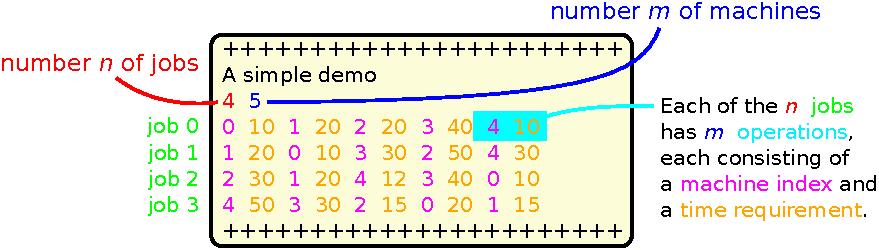
\includegraphics[width=0.9\linewidth]{\currentDir/jssp_demo_instance}%
\caption{The meaning of the text representing our \instStyle{demo} instance of the JSSP, as an example of the format used in the OR-Library.}%
\label{fig:jssp_demo_instance}%
\end{figure}

In the simple text format used in OR-Library, several problem instances can be contained in one file.
Each problem instance~\instance\ starts and ends with a line of several \texttt{+} characters.
The next line is a short description or title of the instance.
In the third line, the number~\jsspJobs\ of jobs is specified, followed by the number~\jsspMachines\ of machines.
The actual IDs or indexes of machines and jobs are 0-based, similar to array indices in Python.
The JSSP instance definition is completed by~\jsspJobs\ lines of text, each of which specifying the operations of one job~$\jsspJobIndex\in\intRange{0}{(\jsspJobs-1)}$.
Each operation~\jsspMachineIndex\ is specified as a pair of two numbers, the ID~$\jsspOperationMachine{\jsspJobIndex}{\jsspMachineIndex}$ of the machine that is to be used (violet), from the interval~$\intRange{0}{(\jsspMachines-1)}$, followed by the number of time units~$\jsspOperationTime{\jsspJobIndex}{\jsspMachineIndex}$ the job will take on that machine.
The order of the operations defines exactly the order in which the job needs to be passed through the machines.
Of course, each machine can only process at most one job at a time.

In our demo instance illustrated in \autoref{fig:jssp_demo_instance}, this means that we have~$\jsspJobs=4$ jobs and~$\jsspMachines=5$ machines.
Job~0 first needs to be processed by machine~0 for 10~time units, it then goes to machine~1 for 20~time units, then to machine~2 for 20~time units, then to machine~3 for 40~time units, and finally to machine~4 for 10~time units.
This job will thus take at least~100 time units to be completed, if it can be scheduled without any delay or waiting period, i.e., if all of its operations can directly be processed by their corresponding machines.
Job~3 first needs to be processed by machine~4 for 50~time units, then by machine~3 for 30~time units, then by machine~2 for 15~time units, then by machine~0 for~20 time units, and finally by machine~1 for 15~time units.
It would not be allowed to first send Job~3 to any machine different from machine~4 and after being processed by machine~4, it must be processed by machine~3 --- although it may be possible that it has to wait for some time, if machine~3 would already be busy processing another job.
In the ideal case, job~3 could be completed after 130~time units.
\endhsection%
%
\hsection{A Python Class for JSSP Instances}%
This structure of a JSSP instance can be represented by the simple Python class.
In \autoref{lst:jssp_instance}, we give an excerpt of this class, i.e., a snippet of the original code where some methods and data verification has been omitted.
Each instance has a \codeil{name}, a number~$\jsspJobs$ of jobs stored in the variable \codeil{jobs}, and a number~$\jsspMachines$ machines stored in the variable \codeil{machines}.
We derive our class from \href{https://numpy.org/doc/stable/reference/generated/numpy.ndarray.html}{\codeil{numpy.ndarray}}, so that it can represent the data directly.
While the text file format displayed in \autoref{fig:jssp_demo_instance} lists the data in two dimensions, we choose to use three:
Each \codeil{Instance} is an array with one row for each job, one column for each operation, and each cell holds two values with the machine and the time spent on the machine.
In other words, an $\instance[\jsspJobIndex, \jsspMachineIndex, 0]$ holds the machine~$\jsspOperationMachine{\jsspJobIndex}{\jsspMachineIndex}$ for the operation~$\jsspMachineIndex$ of job~$\jsspJobIndex$.
$\instance[\jsspJobIndex, \jsspMachineIndex, 1]$ holds the time~$\jsspOperationTime{\jsspJobIndex}{\jsspMachineIndex}$ that job~$\jsspJobIndex$ will spend on machine~$k$.

\moptipyCode{moptipy/examples/jssp/instance.py}{--labels book --args doc,hints,comments}{jssp_instance}{Excerpt from a Python class for representing the data of a JSSP instance.}

We add a static method \codeil{from_resource(name)} to this class that can load any of the aforementioned benchmark JSSP instances directly based on its name.
This way, we can conveniently access all the necessary data of a job shop scheduling task.
The actual code of the above, other utility methods, as well as sanity checks in the \codeil{__new__} constructor have here been omitted as they are unimportant for the understanding of the scenario.%
\endhsection%
\endhsection%
%

